\chapter{Experiments and Results}\label{experiments}
This chapter presents the experiments conducted to evaluate the methods presented in~\Cref{methods}, as well as their set up and the experimental methodology used. The results of each experiment are then presented and discussed in brief.~\Cref{exp_meth} will present the experimental setup used in this thesis, including the choices of metrics, datasets, models used throughout all of the experiments. Baseline generalizability metrics are then collected in~\Cref{models}. The impact of data augmentation on generalization is then tested in~\Cref{augmentations}, which in turn is used as a basis for the experiments performed in~\Cref{consistency_training}, wherein the best augmentation method was selected for use in Consistency Training. Finally, the impact of ensembles is tested in~\Cref{ensembles}. All experiments where conducted using Nvidia Tesla-V100 GPUs on the eX3 computing infrastructure offered by Simula Research Laboratory. The experiments were implemented in Python 3.8 using PyTorch. The source code as well as all of the raw data is available on the GitHub repository given in~\Cref{code_data}.

\section{Experimental Setup}\label{exp_meth}
The experiments conducted in this chapter were partially exploratory and partially quantitative in nature. The relative impacts of the methods and baselines on generalization was determined quantitatively where possible through fitting statistical tests depending on the required null-hypothesis and nature of the distribution within the respective groups. Where further analysis was necessary and feasible, these results were then explored in an attempt to relate them to the theory as presented in \Cref{gen_theory}. 

In addition to exploring the impact of the methods as outlined in~\Cref{methods}, the effects of more well-known methods were also compared. In particular, the effect of the choice of model architecture, the use of data augmentation, and ensemble models was quantified and related to one another. This was then in turn compared to the impact due to the methods presented in \Cref{methods}. 

An alpha-value of 0.01 was used to ascertain statistical significance throughout this thesis. The p-values for all comparisons performed in this thesis can be found in~\Cref{p-values}. The statistical tests used in this thesis are as follows:
\begin{itemize}
    \item Two-sided independent-sample t-tests were used to perform comparisons between approximately normally distributed groups.
    \item The Mann-Whitney U-test was used to perform comparisons between groups that were not normally distributed, for instance when considering the results across multiple models and/or datasets simultaneously.
    \item The Spearman's rank correlation test was used to identify correlations, and was selected due to the lack of assumptions of linearity.
\end{itemize}

The following sections will further detail the experimental setup, including the choices of metrics, datasets, and the choice of models with which the impact of the presented methods were established. 
   \subsubsection{Datasets} \label{datasets}
    Naturally, the best way to evaluate the generalizability of a given predictor is to test it directly on \gls{ood} data. Though this can to some extent be achieved by carefully designing stress-tests ~\cite{damour2020underspecification}, a more straight-forward approach is to simply leverage existing \gls{ood} datasets. To this end, a number of polyp-segmentation datasets were selected. The names, sizes, resolutions and availabilities of these datasets is shown in~\Cref{tab:datasets}. Samples images and masks from the datasets can be seen in~\Cref{fig:dataset_examples}
    
    \begin{table}[htb]
        \centering
       \begin{tabularx}{\linewidth}{lXXX}
        \toprule
        Dataset & Resolution & Size & Availability \\
        \midrule
        Kvasir-SEG ~\cite{kvasir} & Variable & 1000 & Public \\
        Etis-LaribDB ~\cite{etis-larib} & 1255x966 & 196  & Public \\
        CVC-ClinicDB ~\cite{cvc-clinic} & 388x288 & 612  & Public \\
        EndoCV2020 ~\cite{endocv2020} & Variable & 127  & Request \\
        \bottomrule
    \end{tabularx}
        \caption{Dataset Overview}
        \label{tab:datasets}
    \end{table}
    
    \begin{figure}[htb]
        \centering
        \includegraphics[width=\linewidth]{illustrations/dataset_samples.png}
        \caption{Sample images from the datasets.}
        \label{fig:dataset_examples}
    \end{figure}
    
    Ideally, the datasets used in EndoCV2021 ~\cite{endocv2021} should also have been included to facilitate for direct comparison to the results published in the EndoCV2021 proceedings, however since they were not available - neither publically nor by request - at the time of writing this thesis, this was, unfortunately, not possible. 
    
    Kvasir-SEG was selected for being used as the \gls{ind} dataset across all experiments due to its size and the diversity of images. This was then split into a training, validation and test-set, which remained constant across all experiments. The remaining datasets were used solely for \gls{ood} evaluation.
    
    All images were resized to 512x512 as preprocessing during all training runs, as some of the models required base-2 dimensionality.
    
\subsection{Metrics} \label{metrics}
    This subsection will present the metrics used in order to evaluate the performance of the predictors presented in this thesis. As the primary focus is to evaluate generalizability, only two metrics are used, namely mean \gls{iou} and the \glsfirst{cs} of the \gls{iou}.

    \subsubsection{Mean Intersection-over-Union}
    
    The most natural way to quantify generalizability is to simply evaluate the predictors on in-distribution and out-of-distribution data and then consider the differences. There are, naturally, several performance measures that can be used to this end in the context of segmentation, the most natural of which being \gls{iou} or the Dice coefficient, which as discussed in \Cref{background} are equivalent. In this thesis, \gls{iou} was used. To reiterate, IoU is defined as follows:
    Let \(y\) be the segmentation label, and \(\hat{y}=f(x)\) be the segmentation prediction given the model \(f\) and an input image x. The \gls{iou} can then be expressed as: 
    \begin{equation*}
        IoU(y, \hat{y}) = \frac{\sum \{y=\hat{y}\} }{\sum \{y=1\} \cup \{\hat{y}=1\}\}}
    \end{equation*}
    
    Measuring the average \gls{iou} scores across a number of different datasets should, naturally, provide an indication of the generalizability of the given predictor. Though it is of course impossible to account for all distributional shifts that may occur in deployment, high degrees of generalization across multiple datasets should nevertheless translate well to other datasets. 

    
    \subsubsection{Performance Variability}
    As discussed in~\Cref{background}, the prevalence of generalization failure is often attributed to the notion of underspecification. Underspeficified pipelines are characterized by the fact that they can return any number of different predictors, which though all exhibiting more or less identical performance in \gls{ind} settings, learn differing and often conflicting features and thus may differ wildly in \gls{ood} settings. 
    
    To analyze this, the literature tends to consider the performance variability of a set of multiple identically trained predictors ~\cite{damour2020underspecification}.  
    
    One simple approach to quantify this is to take the standard deviation of the mean \gls{iou} scores for the given datasets and predictors. This, however, implicitly rewards predictors that perform poorly. To mitigate this, the \gls{cs} can instead be used. \gls{cs} is similar to the standard deviation, but normalized by the mean. This is shown in \Cref{cstd}, where \(n=|\{x_0, x_1, \ldots, x_n\}|\) is the number of samples (in this thesis: mean \gls{iou} for a given predictor), and \(\mu\) is the sample mean (in this thesis: the mean of the mean \glspl{iou} across predictor samples)
    \begin{equation}\label{cstd}
        C.StD = \frac{1}{n \mu} \sqrt{ \sum_i^n (\mu - x_i)^2  }
    \end{equation}
    
     Though the mean generalizability gap across these predictors is the primary indication of generalizability of the pipeline, this variability is also a salient factor to consider as it serves to quantify the degree to which a given pipeline is underspecified. The more underspecified a pipeline is, the higher the variability of the performance and the higher the \gls{cs} of the \glspl{iou}.  

\subsection{Models} \label{model_choices}
In order to evaluate the impact of the methods presented in~\Cref{methods} sufficiently, they need to be tested across a range of different models. This ensures that the effects induced my the methods are not model-dependent, and in addition provides an opportunity to investigate the innate ability of specific models to learn generalizable features. To this end, a number of popular models were selected, intended to serve as a somewhat representative sample of what may be considered as "typical" deep learning pipelines. These models include DeepLabV3+ ~\cite{deeplab}, \gls{fpn} ~\cite{fpn}, UNet ~\cite{unet}, Tri-Unet ~\cite{divergentnets}, and the dual-decoder DeepLabV3+ as introduced in \Cref{methods}. 

The models were implemented in pytorch using the segmentation-models-pytorch (SMP) library ~\cite{smp}, using the library's default values.~\Cref{tab:baselines} shows the architecture type and parameter counts of the respective models. 
  \begin{table}[htb]
            \centering
            \begin{tabularx}{\linewidth}{lXr}
            \toprule
                 Model & Architecture & Parameters  \\
            \midrule
                 UNet ~\cite{unet} & Encoder-Decoder & 48872738\\ 
                 TriUnet ~\cite{divergentnets} &
                 Stacked Encoder-Decoder & 122178709\\
                 FPN ~\cite{fpn} & Pyramidal & 47591762\\ 
                 DeepLabV3+ ~\cite{deeplab} & Hybrid & 22437457\\ 
                 Dual Decoder DeepLabV3+& Single-encoder Dual-decoder & 23590756\\
            \bottomrule
            \end{tabularx}
            \caption{Experiment Models}
            \label{tab:baselines}
        \end{table}
The models were all intialized using SMP's built-in pretrained weights, trained on ImageNet. Though foregoing pretraining would perhaps highlight the respective models' innate generalization ability to a greater extent, the use of pretrained weights nonetheless constitutes a more realistic context, as most computer vision pipelines, especially those of a medical nature, employ some form of pretraining. As will be discussed in~\Cref{discussion}, evaluating the generalizability of different models without pretraining may however be an interesting direction of further study. 
 

\section{Model Architecture} \label{models}
To establish the effect of model architectures alone, ten predictors were trained for each model without augmentation and using regular Jaccard loss, according to the hyperparameters shown in~\Cref{table:hyperparameters}. 
\begin{table}[htb]
        \centering
        \begin{tabularx}{\linewidth}{llX}
        \toprule
        \multicolumn{3}{c}{\textbf{Pipeline Configuration}}\\
        \toprule
        Component & Type & Hyperparameters \\
        \midrule
        Dataloader & - & \(batch\_size = 8\) \\
        && \(\hbox{train/val/test split} = 80/10/10\)\\
        \midrule
        Optimizer & Adam & \(lr = 0.00001\)\\
        \midrule
        Scheduler & Cosine Annealing w/ Warm Restarts & \(T_0=50\) \\
        & & \(T_{mult}=2\) \\
        \midrule
        Evaluation & Loss-based Early Stopping & \(epochs=300\)\\
        \bottomrule
        \end{tabularx}
            \caption{Hyperparameters for baselines}
            \label{table:hyperparameters}
\end{table}

The mean \glspl{iou} for each dataset are shown in~\Cref{tab:baseline_iou}. Though the differences between many pairs of models are statistically significant for several datasets, the magnitude thereof is marginal to the point of being inconsequential for practical purposes, with the exception of TriUnet which exhibited considerably worse generalization. All p-values are shown in~\Cref{models_pvalues}.

\begin{table}[htb]
    \centering
    \small
    \begin{tabularx}{\linewidth}{@{}lXXXX@{}}
    \toprule
    & Kvasir-SEG & Etis-LaribDB & CVC-ClinicDB & EndoCV2020 \\
    \midrule
    DeepLabV3+ & 0.819 & \textbf{0.412}  & 0.678 & 0.604 \\
    DD-DeepLabV3+ &\textbf{0.832} & 0.406 & \textbf{0.683} & 0.595 \\
    Unet & 0.828 & 0.403 & 0.679 & 0.599 \\
    TriUnet & 0.822 & 0.305 & 0.633 & 0.581 \\
    FPN& 0.823 & 0.404 &0.678 & \textbf{0.605}\\
    \bottomrule
    \end{tabularx}
.    \caption[Mean IoU scores for each model across datasets]{Mean IoU scores for each model across datasets. The best models for each dataset are highlighted in bold.}
    \label{tab:baseline_iou}
\end{table}

\Cref{fig:baseline_ious} shows the models' average change in mean \gls{iou} across the three \gls{ood} datasets with respect to the mean \gls{iou} of the \gls{ind} dataset. All models exhibited considerable performance degradation, as expected per the discussion in \Cref{case_studies}. Once again, the  differences across architectures are fairly marginal, once again with the exception of the TriUnet. 
    \begin{figure}[htb]
        \centering
        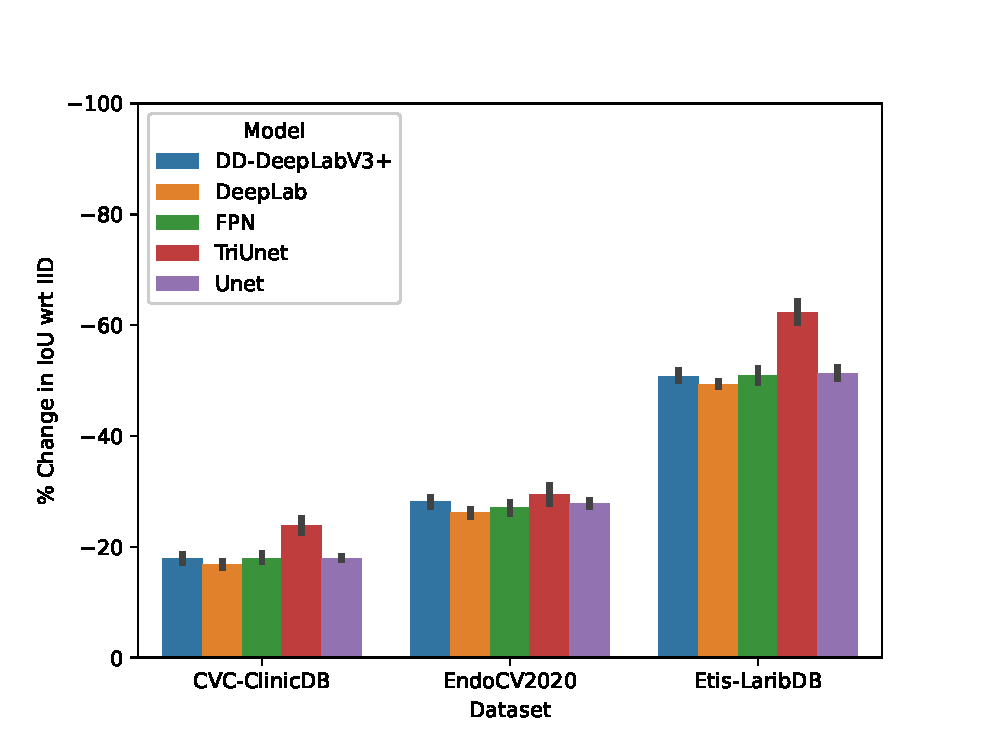
\includegraphics[width=\linewidth]{illustrations/delta_iou_baseline.eps}
        \caption{Change in \gls{ood} \gls{iou} as a percentage of the \gls{ind} \gls{iou} across models and datasets.}
        \label{fig:baseline_ious}
    \end{figure}

    What differences there are across the models, however, can to some extent be understood according to the extent to which the models are underspecified.~\Cref{fig:baseline_cstd} shows the \gls{cs} values for each model and dataset as computed from the evaluation of the ten predictors. 
    
    \begin{figure}[htb]
        \centering
        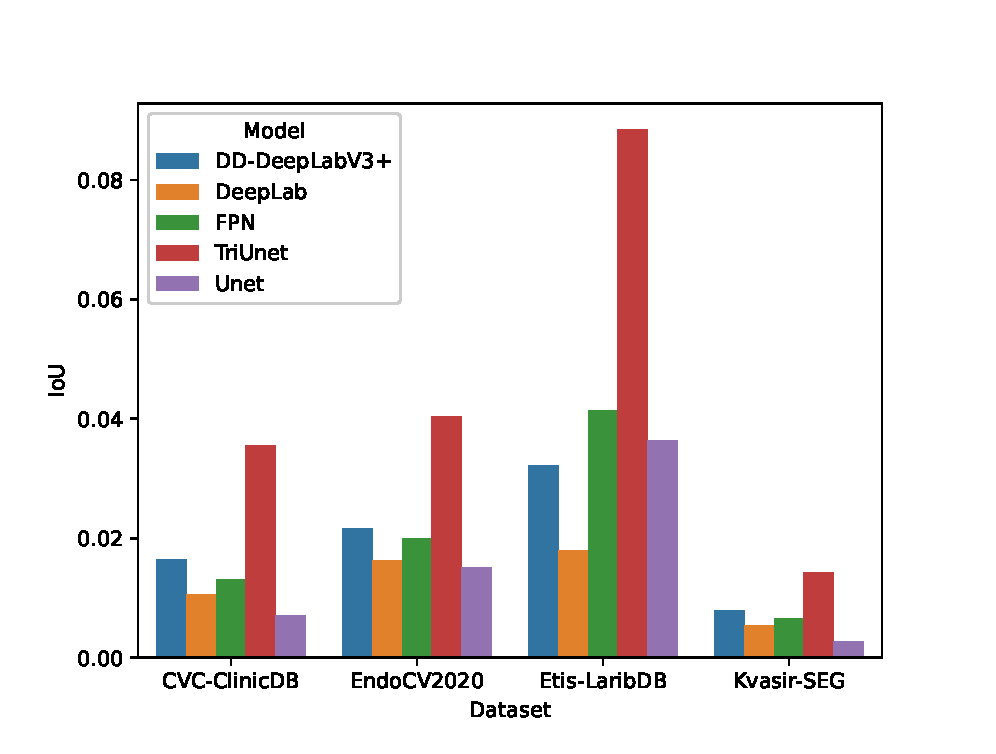
\includegraphics[width=\linewidth]{illustrations/cstd_baseline.eps}
        \caption{Coefficient of Standard Deviation across models and datasets.}
        \label{fig:baseline_cstd}
    \end{figure}
    
    Evidently, the margins seperating the models in terms of  mean \gls{iou} are similar to the margins sepearating the models in terms of the \gls{cs}. 
    
    Indeed, as is shown in \c there is a strong correlation between the two metrics, suggesting that underspecification plays a considerably more significant role than the model architectures themselves. I.e, the more underspecified the model is, the greater the falls in \gls{iou} on \gls{ood} datasets. 
    
    \begin{figure}[htb]
        \centering
        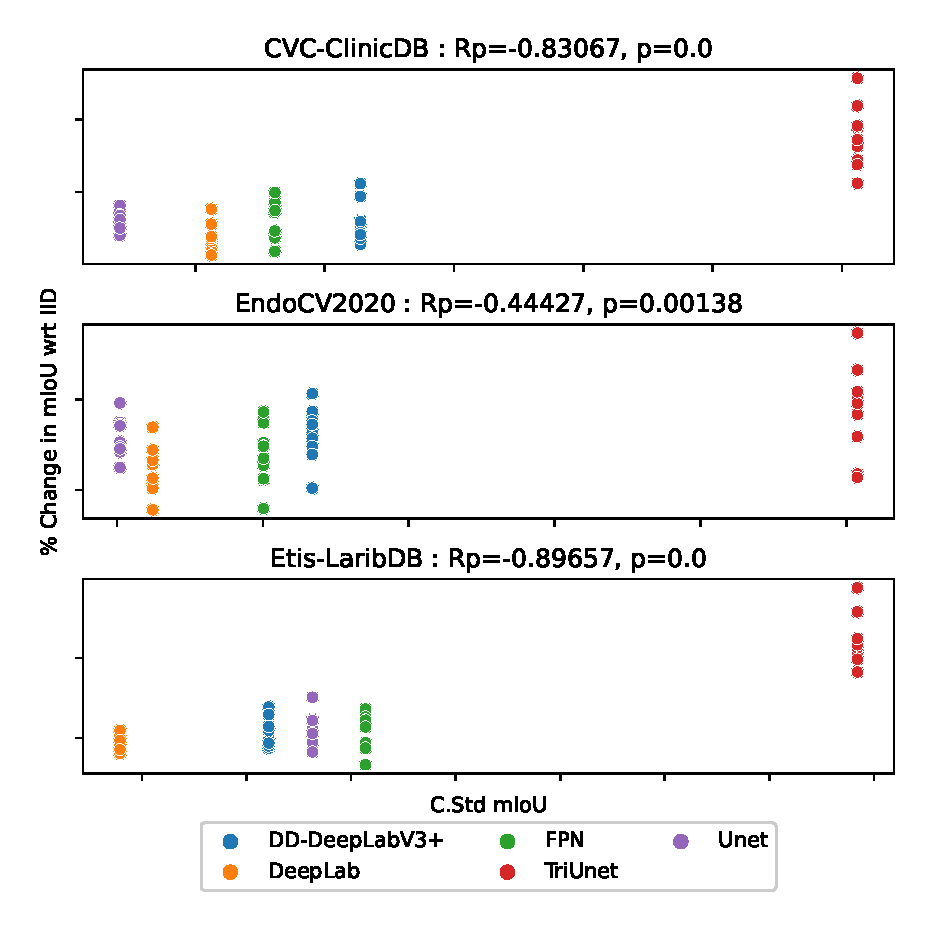
\includegraphics{illustrations/underspecification_baseline.eps}
        \caption[Correlation between Generalizability and Underspecification]{Scatter-plot showing the relationship between model underspecification as quantified by \gls{cs} and generalization failure as quantified change in mean \gls{iou} as a percentage of the \gls{ind} \gls{iou}.}
        \label{fig:my_label}
    \end{figure}

    Of particular interest is the relationship between the Unet and the TriUNet, as well as DeepLabV3+ and the dual-decoder counterpart. The differences between these two pairs of models will be discussed in further depth below.
    
    \subsubsection{Unet vs TriUnet}
    Consider the differences between the TriUnet and the Unet as shown in \Cref{fig:baseline_cstd} and \Cref{fig:baseline_ious}. As the TriUnet consists of three UNets, many analyses would assert that the TriUnet should exhibit equivalent performance or greater, as it affords increased support over the regular Unet. However, the results instead demonstrate that the TriUnet on average performs worse than the regular Unet. This can be understood by considering the degree to which the respective models are subject to underspecification. In this thesis, this is quantified by the performance varaibility (\gls{cs}). 
    
    This corroborates the notion that underspecification plays a significant role in generalization failure; the TriUnet is highly underspecified in comparison to the Unet, as the difference in performance variability between shows in~\Cref{fig:baseline_cstd}.
    
    \subsection{DeepLabV3+ vs DD-DeepLabV3+} \label{dd-deeplab}
    DeepLabV3+ and DD-DeepLabV3+ both exhibited more or less comparable performance when considering their \gls{ood} IoUs, as shown in~\Cref{tab:baseline_iou}. Interestingly, though, the dual-decoder model performed better on the \gls{ind} dataset - Kvasir-Seg - by a statistically significant margin (p<0.01). There are also some differences with regards performance variability, albeit minor. As shown in~\Cref{fig:baseline_cstd}, the DD-DeepLabV3+ exhibits lower \gls{cs} scores than its single-decoder counterpart. Since the models are as mentioned functionally identical except for the presence of the reconstruction decoder during the training of DD-DeepLabV3+, this can only be attributed to the model learning a more limited latent representation and thus being less underspecified. 
    
    \begin{figure}[htb]
        \centering
        \includegraphics[width=\linewidth]{illustrations/reconstruction_samples.png}
        \caption{Reconstruction Examples across datasets}
        \label{fig:reconstruction}
    \end{figure}

    The differences between the two models are smaller than expected, however. One possible explanation for this may be that segmentation encoders learn somewhat task-agnostic representations of the data by default, and that the presence of a reconstruction decoder merely refines these representations to a minor extent, however in a manner that does not meaningfully affect the segmentation task. This notion is supported by the fact that the reconstruction seems to be equally good in terms of L1-distance across all four datasets. If the encoder had learned dataset-specific features, this would not be the case. A histogram showing the distribution of L1-scores across the four dataset is shown in~\Cref{fig:l1_rec}. Reconstruction examples are shown in~\Cref{fig:reconstruction}. Most of the errors seem to cluster around areas of high reflectivity regardless of dataset.  
    
    \begin{figure}[htb]
        \centering
        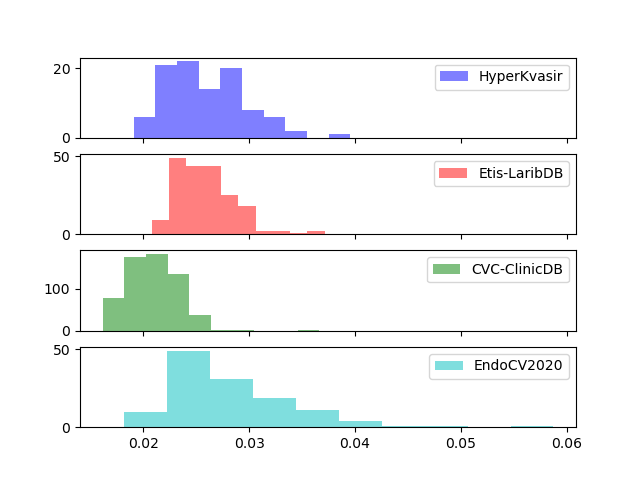
\includegraphics[width=\linewidth]{illustrations/l1_reconstruction.png}
        \caption[L1 reconstruction distributions across datasets]{Distribution of L1 reconstruction scores across datasets. Though the distributions vary, there is no clear evidence of generalization failure in terms of reconstruction.}
        \label{fig:l1_rec}
    \end{figure}
    

\section{Augmentation Strategies}\label{augmentations}
The baseline predictors collected in the previous section were then compared to predictors trained using data augmentation. Two augmentation strategies were tested: one with conventional augmentations only, while the other also incorporates the GAN-inpainter. The models were trained according to the same hyperparameters as described in~\Cref{table:hyperparameters}. The data augmentation strategy was implemented using the albumentations library, and the hyperparameters were tuned according to the methods referred to in~\Cref{methods}. The data was then augmented with a probability of 0.5, in which case the constituent transformations were applied according to the ranges defined by the hyperparameters. The results for each configuration and across models and datasets are shown in~\Cref{tab:aug_ious}.

\begin{table}[htb]
    \centering
\begin{tabularx}{\linewidth}{lXXX}
\toprule
Model & No Augmentation & Vanilla Augmentation & Inpainter+Vanilla Augmentation\\
\midrule
\multicolumn{4}{c}{\textbf{Kvasir-SEG }}\\
\midrule
           DD-DeepLabV3+     & 0.829 & \textbf{0.848} & 0.844\\
           DeepLabV3+        & 0.822 & \textbf{0.850} & 0.846\\
           FPN               & 0.822 & \textbf{0.853} & 0.848\\
           TriUnet           & 0.817 & 0.841          & \textbf{0.842}\\
           Unet              & 0.828 & \textbf{0.851} & 0.846\\
\midrule
\multicolumn{4}{c}{\textbf{Etis-LaribDB}}\\
\midrule
           DD-DeepLabV3+     & 0.408 & \textbf{0.460} & 0.435\\
           DeepLabV3+        & 0.417 & \textbf{0.472} & 0.451\\
           FPN               & 0.404 & \textbf{0.440} & 0.422\\
           TriUnet           & 0.309 & \textbf{0.410} & 0.382\\
           Unet              & 0.403 & \textbf{0.447} & 0.414\\
\midrule
\multicolumn{4}{c}{\textbf{CVC-ClinicDB}}\\
\midrule

           DD-DeepLabV3+     & 0.681 & \textbf{0.728} & 0.713\\
           DeepLabV3+        & 0.684 & \textbf{0.733} & 0.718\\
           FPN               & 0.675 & \textbf{0.715} & 0.705\\
           TriUnet           & 0.623 & \textbf{0.684} & 0.659\\
           Unet              & 0.679 & \textbf{0.717} & 0.703\\
\midrule
\multicolumn{4}{c}{\textbf{EndoCV2020}}\\
\midrule
           DD-DeepLabV3+     & 0.596 & \textbf{0.668} & \textbf{0.668}\\
           DeepLabV3+        & 0.608 & \textbf{0.676} & 0.670\\
           FPN               & 0.600 & \textbf{0.662} & 0.661\\
           TriUnet           & 0.577 & \textbf{0.667} & 0.656\\
           Unet              & 0.598 & 0.660          & \textbf{0.665}\\
\bottomrule
\end{tabularx}
    \caption[Mean IoUs across augmentation strategies grouped by model and dataset.]{Mean IoUs across augmentation strategies grouped by model and dataset. The best augmentation strategy for each dataset and model are highlighted in bold. }
    \label{tab:aug_ious}
\end{table}

Both augmentation strategies exhibit an increase in \gls{ood} performance when compared to the baseline, i.e no augmentation (p<0.01). Averaged across models, the predictors trained using both conventional augmentations and the inpainter perform worse than the predictors trained with the conventional augmentations only on Etis-LaribDB and CVC-ClinicDB (p<0.01). There appear to be insignificant differences for the remaining two datasets. The p-values for each dataset can be found in~\Cref{tab:ttest_avgs_inpainter}. When considering each model individually, the differences are statistically insignificant, though this can be attributed to the low sample size. The p-values for this can be found in~\Cref{tab:ttest_per_dataset_inpainter}. 

The relative improvements due to the two augmentation strategies as a percentage of the mean \gls{iou} of the baselines is shown in~\Cref{fig:augmentations}. 

\begin{figure}[htb]
    \centering
    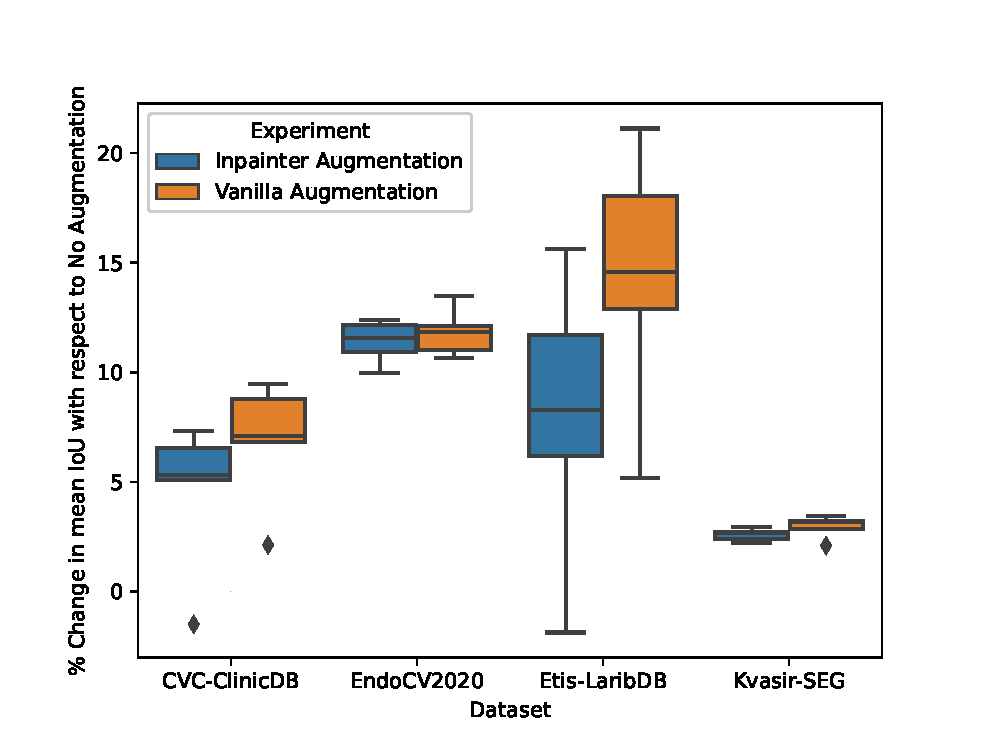
\includegraphics[width=\linewidth]{illustrations/augmentation_plot.eps}
    \caption[Augmentation Improvements]{Strip Plot of the ensembles' improvements in \gls{iou} per dataset as a percentage of the mean \gls{iou} of the corresponding model.}
    \label{fig:augmentations}
\end{figure}

The difference between the three augmentation strategies is best highlighted by the models' performance on Etis-LaribDB, the most difficult of the three \gls{ood} datasets, which exhibits increases in mean \gls{iou} of 7.99\% using the inpainter and conventional augmentation and 14.35\% using only conventional augmentation. The differences are slightly less pronounced on the CVC-ClinicDB dataset, now with mean \gls{iou} improvements of 4.55\% AND 6.86\& respectively, and negligible on the two remaining datasets. One possible reason for this is that the inpainter may have learned \gls{ind}-specific features, and thus increase the models' bias towards learning these types of features. One can to a minor extent argue that this may explain the limited difference between the two aforementioned augmentation strategies in the \gls{ind} dataset, i.e KvasirSeg. However, it does not seem to affect the performance on the EndoCV2020 dataset by any significant margin either. One possible explanation for this is that the polyps look similar in both datasets, but verifying this requires further experimentation. 

Regardless, it is clear that synthetic augmentation as implemented in this thesis does not benefit generalization. As will be discussed in~\Cref{discussion}, however, the results do not however conclusively prove the inefficacy of \gls{ind}-trained \glspl{gan} for augmentation as a whole, only that it is unlikely that the implementation in this thesis is particularly useful. 


\section{Consistency Training}\label{consistency_training}
Though data augmentation on its own increases generalizability by virtue of the fact that it increases the support of the model, it does not explicitly impose any inductive biases, and as discussed in~\Cref{methods} may not be sufficient to impose invariance to the relevant transformations. To address this, Consistency Training was introduced. To reiterate, Consistency Training requires a perturbation model - in practical terms, an augmentation strategy - and a loss function that quantifies the degree to which the model is inconsistent to these perturbations, which for the segmentation task is implemented as \gls{sil}. In the previous section, it was established that conventional augmentations are the most conducive to generalization. Thus, this augmentation strategy was chosen as the perturbation model. 

For each model architecture, ten predictors were trained using Consistency Training, once again using the same hyperparameters as shown in~\Cref{table:hyperparameters}. This was then compared to the predictors trained using the conventional pipeline with the same augmentation strategy, as Consistency Training is as discussed in practical an alternative to conventional augmentation, and to predictors trained without augmentation. The \glspl{iou} for this experiment are shown in~\Cref{tab:aug_ious}.

\begin{table}[htb]
    \centering
\begin{tabularx}{\linewidth}{llXX}
\toprule
\textbf{Model} & \textbf{No Augmentation} & \textbf{Vanilla Augmentation} & \textbf{Consistency Training}\\
\toprule
\multicolumn{4}{c}{\textbf{Kvasir-SEG  }}\\
\midrule

        DD-DeepLabV3+& 0.829 & 0.848 & \textbf{0.852} \\
        DeepLab& 0.822 & 0.850 & \textbf{0.852} \\
        FPN& 0.822 & \textbf{0.853} & 0.852 \\
        TriUnet& 0.817 & 0.841 & \textbf{0.845} \\
        Unet& 0.828 & \textbf{0.851} & \textbf{0.851} \\
\midrule
\multicolumn{4}{c}{\textbf{Etis-LaribDB}}\\
\midrule
        DD-DeepLabV3+& 0.408 & 0.460 & \textbf{0.482 }\\
        DeepLab& 0.417 & 0.472 & \textbf{0.505}* \\
        FPN& 0.404 & 0.440 & \textbf{0.475}* \\
        TriUnet& 0.309 & 0.410 & \textbf{0.434} \\
        Unet& 0.403 & 0.447 & \textbf{0.481}* \\
\midrule
\multicolumn{4}{c}{\textbf{CVC-ClinicDB}}\\
\midrule
        DD-DeepLabV3+ & 0.681 & 0.728 & \textbf{0.736} \\
        DeepLabV3+& 0.684 & 0.733 & \textbf{0.740} \\
        FPN& 0.675 & 0.715 & \textbf{0.727}* \\
        TriUnet& 0.623 & 0.684 & \textbf{0.696} \\
        Unet& 0.679 & 0.717 & \textbf{0.730}* \\
\midrule
\multicolumn{4}{c}{\textbf{EndoCV2020}}\\
\midrule
        DD-DeepLabV3+& 0.596 & \textbf{0.668} & \textbf{0.668} \\
        DeepLab& 0.608 & \textbf{0.676} & \textbf{0.676} \\
        FPN& 0.600 & 0.662 & \textbf{0.673 }\\
        TriUnet& 0.577 & 0.667 & \textbf{0.684} \\
        Unet& 0.598 & 0.660 & \textbf{0.676}*\\
\bottomrule
    \end{tabularx}
    \caption[Mean IoUs for training methods]{Mean IoUs for training methods, precision truncated to 99\% confidence. Consistency Training entries with greater performance than conventional augmentation by for the given model and dataset are highlighted in bold. If statistically significant after a two-tailed independent sample t-test, they are also marked with a "*"}
    \label{tab:consistency}
\end{table}

The results show that Consistency Training increases generalization considerably, outperforming data augmentation by a statistically significant margin when averaging across models on all \gls{ood} datasets. This is shown in~\Cref{fig:consistency_training_improvement}. P-values can be found in~\Cref{tab:ttest_avgs_consistency}. 

When analyzing the improvements for the individual models, statistical significance was achieved for all models except the TriUnet on the Etis-LaribDB dataset, for the FPN and Unet on the CVC-ClinicDB dataset, and for the Unet on the EndoCV2020 dataset. The p-values for these comparisons are found in~\Cref{tab:ttest_per_dataset_consistency}. When averaging across models, 
\begin{figure}[htb]
    \centering
    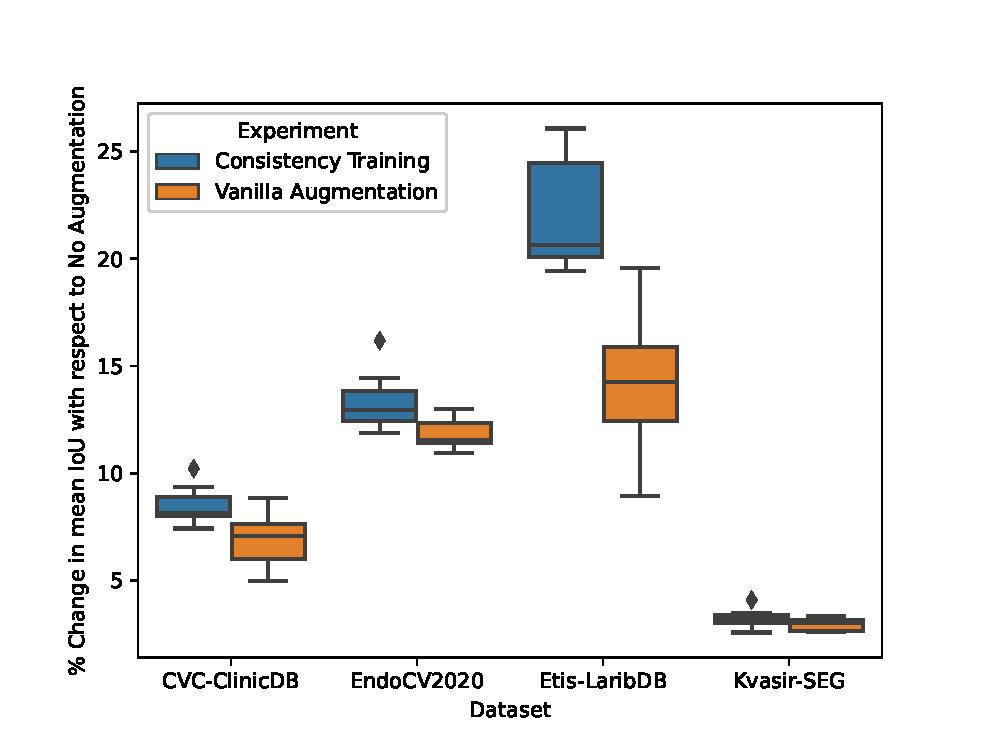
\includegraphics[width=\linewidth]{illustrations/consistency_training_percent.eps}
    \caption[Consistency Training improvements]{Improvements due Consistency Training and Data Augmentation as a percentage the mean \gls{iou} without augmentation across datasets}
    \label{fig:consistency_training_improvement}
\end{figure}

As discussed in~\Cref{cons_vs_aug}, this is to be expected. Consistency training can be interpreted as imposing a more credible set of inductive biases by explicitly optimizing for consistency across augmentations. This is also evidenced by considering the performance variability across the configurations,  shown in~\Cref{fig:consistency_cstd}. Though the relationship between the \glspl{cs} values cannot be confirmed to statistical significance due to the low sample sizes involved in this thesis, a matter that will be discussed further in \Cref{discussion}, 

\begin{figure}[htb]
    \centering
    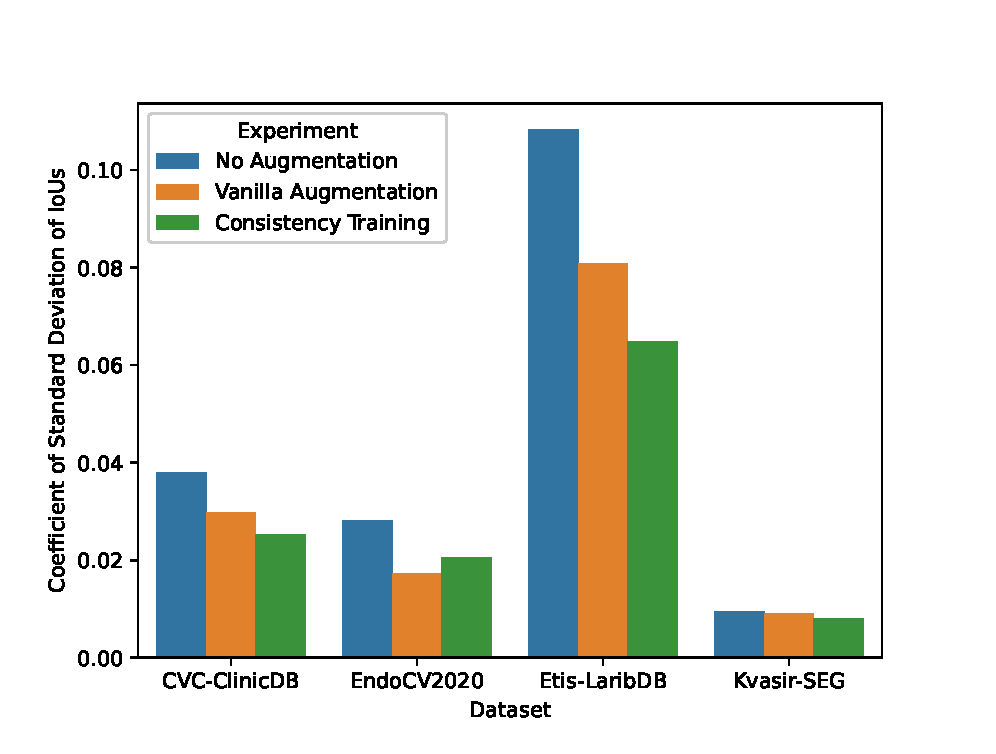
\includegraphics[width=\linewidth]{illustrations/consistency_training_cstd.eps}
    \caption[Consistency Training performance variability]{Models trained with Consistency Training exhibit lower predictor-wise performance variability than models trained without augmentation or with regular data augmentation}
    \label{fig:consistency_cstd}
\end{figure}

\section{Ensembles}\label{ensembles}

Finally, the impact of combining multiple predictors into an ensemble was investigated. Two types of ensembles were investigated: ensembles consisting of five instances of a single type of model and ensembles consisting of all five models. The generalizability of these ensembles were then compared to one another and with the average performance of their constituent predictors. Such analysis was performed across all of the the training-methods tested in \Cref{consistency_training}, i.e. no augmentation, conventional data augmentation, and Consistency Training. Finally, the relationship between the improvement due to ensembles and underspecification was explored. 

To ascertain the generalizability of the ensembles to statistical significance, ten ensembles of each kind were implemented. For the multi-model ensembles, each of the ten ensembles was built from unique predictors trained in~\Cref{consistency_training}.  For the single-model ensembles, five predictors were randomly selected from the ten that were trained in~\Cref{consistency_training}. As will be further discussed in~\Cref{discussion}, these ensembles too should have been built from unique predictors, however due to limits of computational resources this was not possible. 

\subsection{Improvements over Single Models}\label{ensemble_improvement_section}
First, the generalizability of ensemble models was compared to that of the single models. As previously noted, this was performed on pairs of ensembles and single models across all the three training methods compared in \Cref{consistency_training}. The \gls{iou}-scores for the ensemble models are shown in~\Cref{tab:ensembles}. Averaging across models, the ensembles exhibited increased mean \glspl{iou} on all of the \gls{ood} datasets when compared to the mean \gls{iou} of the constituent models as shown in~\Cref{tab:consistency} (p<0.01). See~\Cref{tab:ensemble_v_singular} for p-values. This corroborates the findings in other works that ensembles contribute to increased generalization~\cite{endoensemble, divergentnets}. 
\begin{table}[htb]
    \centering
    \begin{tabularx}{\linewidth}{lXXXr}
\toprule
Ensemble  & CVC-ClinicDB & EndoCV 2020 & Etis-LaribDB & Kvasir-Seg \\
\midrule
\multicolumn{5}{c}{\textbf{Consistency-Trained}}\\
\midrule
DD-DeepLabV3+   & 0.748 &0.684 &0.492 &0.863 \\
DeepLabV3+      & \textbf{0.751} & 0.683 & \textbf{0.523} &0.859 \\
FPN             & 0.739 & 0.685 &0.478 & 0.868 \\
Unet            & 0.744 & 0.694 &0.494 & 0.868 \\
TriUnet         & 0.723 & \textbf{0.715} & 0.468 & 0.859 \\
MultiModel      & 0.747 & 0.693 &0.484 &0.867 \\
\midrule
\multicolumn{5}{c}{\textbf{Conventional Augmentation}}\\
\midrule
DD-DeepLabV3+   & 0.746 & 0.685 & 0.480 & 0.861 \\
DeepLab         & 0.750 & 0.692 & 0.492 & 0.862 \\
FPN             & 0.732 & 0.684 & 0.457 & \textbf{0.869} \\
TriUnet         & 0.715 & 0.692 & 0.440 & 0.860 \\
Unet            & 0.735 & 0.677 & 0.457 & 0.867 \\
MultiModel      & 0.740 & 0.687 & 0.462 & 0.867 \\
\midrule
\multicolumn{5}{c}{\textbf{No Augmentation}}\\
\midrule
DD-DeepLabV3+  & 0.690 & 0.605 & 0.419 & 0.840 \\ 
DeepLab        & 0.695 & 0.611 & 0.426 & 0.833 \\ 
FPN            & 0.690 & 0.610 & 0.416 & 0.837 \\ 
TriUnet        & 0.651 & 0.588 & 0.311 & 0.841 \\ 
Unet           & 0.696 & 0.604 & 0.409 & 0.841 \\
MultiModel     & 0.694 & 0.612 & 0.414 & 0.846 \\
\bottomrule
\end{tabularx}
    \caption[IoUs across ensemble models and datasets. ]{IoUs across ensemble models, datasets, and training methods. Best ensembles for each dataset are highlighted in bold.}
    \label{tab:ensembles}
\end{table}

\begin{figure}[htb]
    \centering
    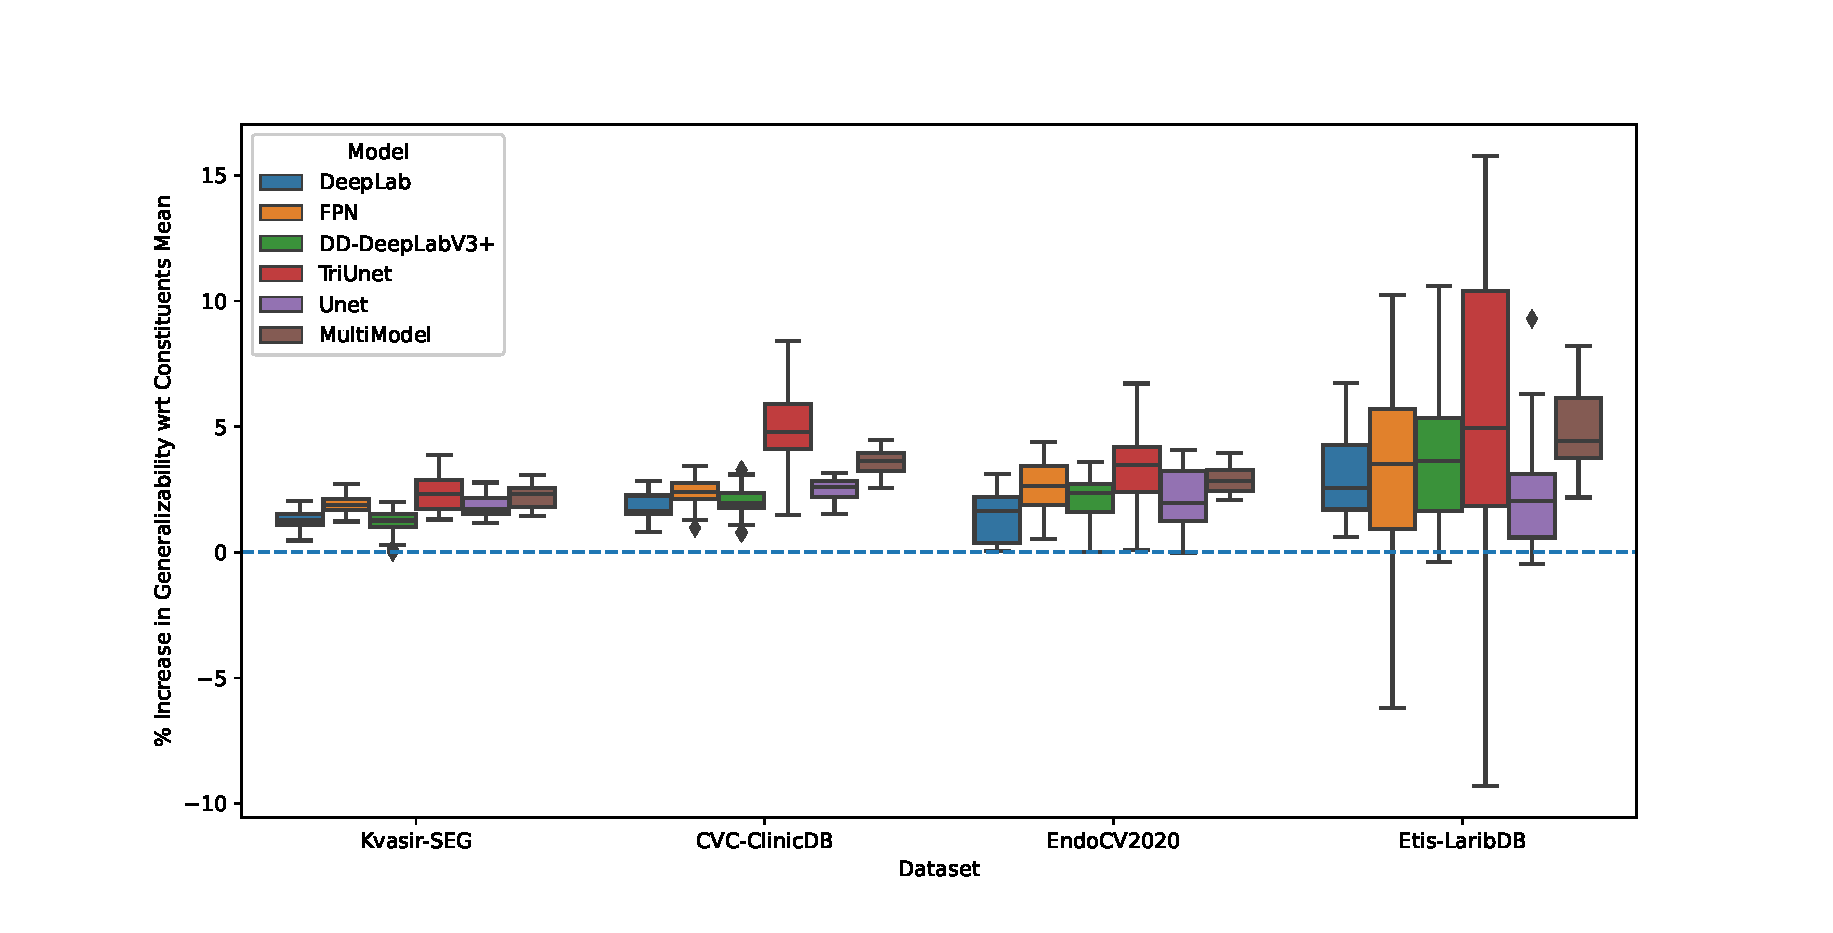
\includegraphics[width=\linewidth]{illustrations/improvements_due_to_ensembles.eps}
    \caption[Improvements due to Ensembles]{Boxplot showing the improvement due to ensembles as a percentage of the mean \gls{iou} across their constituent models across all three training methods}
    \label{fig:ensemble_improvements}
\end{figure}

 
\subsection{Effect of Ensemble Training Methods}\label{ensemble_training_methods}

The difference in \gls{iou} between the three ensemble training methods was statistically significant on all datasets (p<0.01), except CVC-ClinicDB, wherein the difference between the ensembles trained with Consistency Training and the ensembles trained with conventional data augmentation had a p-value of 0.012. The p-values can be found in~\Cref{fig:ttest_training_methods_ensembles}. 

The difference between the relative improvements across the three training methods were statistically insignificant (p>0.01), with the average change in IoU as a percentage of the mean \gls{iou} of the constituent models being 2.026\%, 3.081\% and 2.351\% respectively across all datasets for ensembles trained with no augmentation, conventional augmentation, and Consistency Training.  This is shown in \Cref{fig:ensemble_improvements_across_training_methods}. The p-values are shown in \Cref{fig:ensemble_improvement_tmethod}. 

\begin{figure}
    \centering
    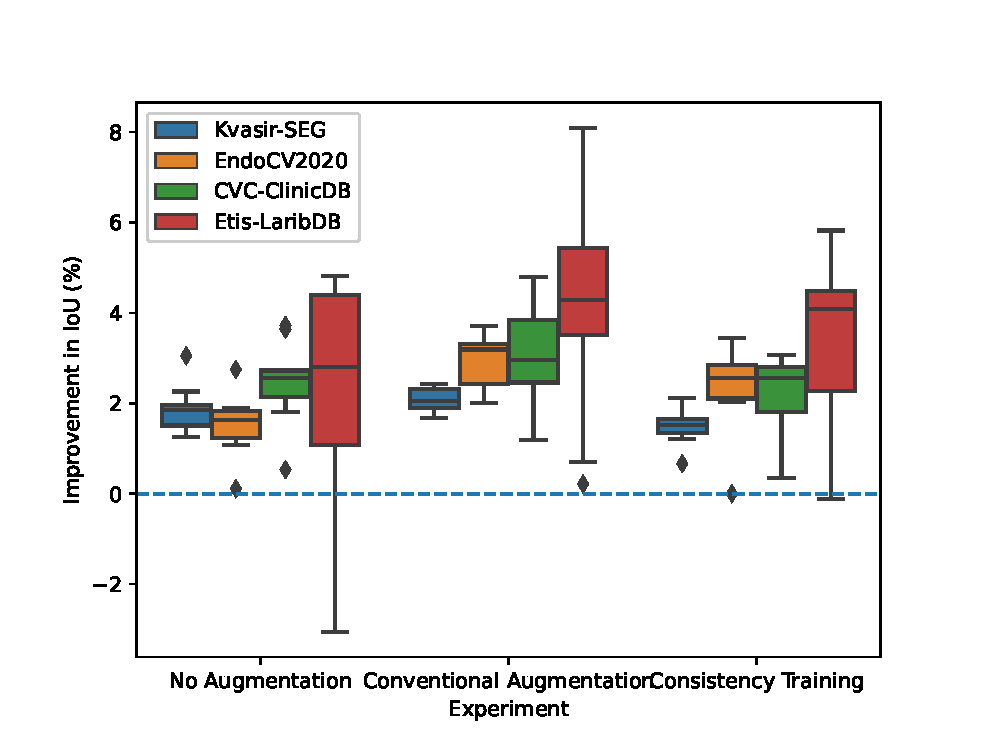
\includegraphics[width=\linewidth]{illustrations/ensemble_improvements.eps}
    \caption[Ensemble improvements across training methods]{Ensemble improvements across training methods and datasets as a percentage of the mean \gls{iou} of the corresponding model architecture}
    \label{fig:ensemble_improvements_across_training_methods}
\end{figure}



To further analyze the impact of ensembles with respect to single models, one can consider the relative performance improvements between them. To this end, the performance of the ensembles trained with Consistency Training was compared to the mean performance of its constituent predictors across all tested model architectures. The relative improvements as a percentage of the constituent predictor performance are shown in~\Cref{fig:ensemble_improvements}. The results show that ensembles increase generalization. However, this is not always the case; perhaps counter-intuitively, the use of ensembles may in certain cases reduce generalization. This occurred on some of the samples of the DD-DeepLabV3+ and FPN-ensembles on Etis-LaribDB, for instance. This may happen when there are high degrees of disagreement among the constituent predictors, in which case there may not be sufficient consensus to fully segment the polyp. Many implementations of ensembles, therein the implementation used in this thesis, require at least a 50\% consensus in order for a given pixel to be classified positively, and thus if this is not achieved, the ensemble may perform worse than any one of the constituent predictors. 

\subsection{Ensembles and Underspecification} \label{ensemble_underspecification}
The tendency of ensembles to increase generalization is as mentioned in~\Cref{background} often attributed to the fact that the use of ensembles to some extent mitigate underspecification. Specifically, they constitute a form of Bayesian marginalization, and should thus in theory be able to leverage the variability of its constituent predictors in order to increase generalization. This assumes that predictions with high consensus are the most generalizable, though as shown in \Cref{fig:bayesian_generalization} this may not be the case. 

To further investigate the veracity of this line of reasoning, one can consider the relationship between the improvements to generalization due to the use of ensembles versus the degree to which the pipelines that generate the constituent predictors are underspecified. This is shown in~\Cref{fig:ensemble_var}. 
\begin{figure}[!hbt]
    \centering
    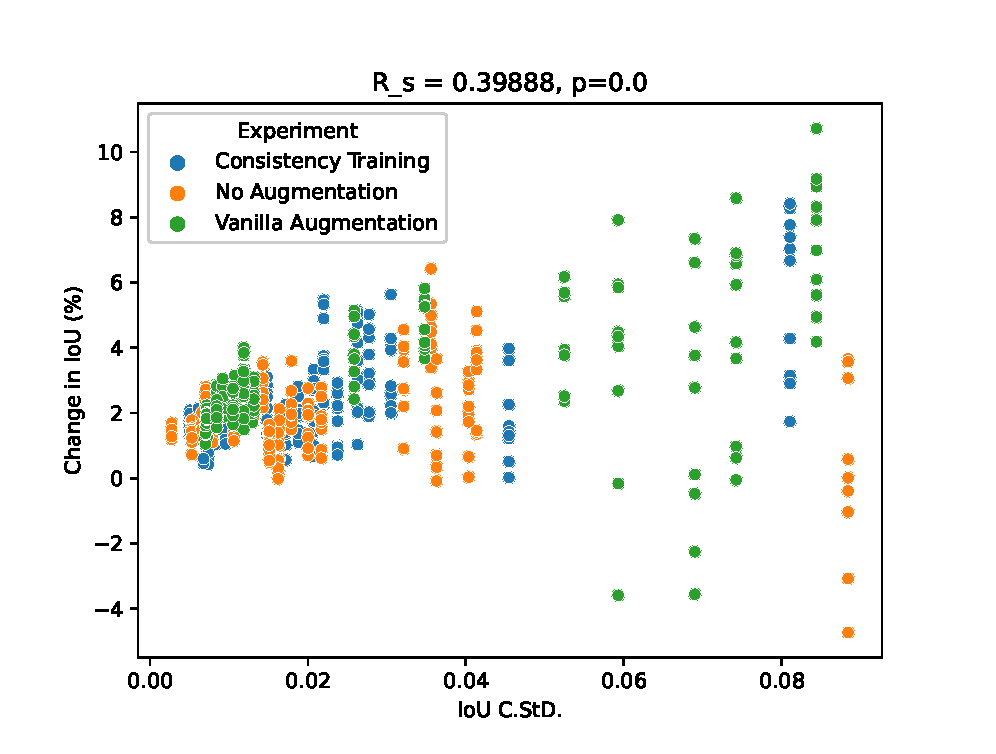
\includegraphics[width=0.9\linewidth]{illustrations/ensembles_underspecification.eps}
    \caption[Relationship between ensemble improvements and underspecification]{Plot showing the relationship between predictor-wise performance variability and improvements in generalization due ensembles trained with Consistency Training. The error-bars show the 99\% confidence intervals for the improvement. The more under specified the pipeline is as quantified by performance variability, the greater improvements are made through the use of ensembles. }
    \label{fig:ensemble_var}
\end{figure}

There appears to be a positive relationship between the two, which corroborates the aforementioned interpretation. It should be noted, however, that the relatively low sample size and consequent potential errors in the estimate for the \gls{cs} means that this relationship cannot be determined with statistical certainty. This will be discussed further in~\Cref{discussion}. 

In~\Cref{fig:ensemble_var}, it should also be noted that the \gls{cs} values are computed based on all ten samples, as it is supposed to represent the degree to which the pipeline itself is underspecified, and not the variability of the constituent predictors for each ensemble instance. One can instead consider the variability in performance of the constituent predictors, which it can be argued is a better representation of the diversity of features learned by the ensembles. This is shown in~\Cref{fig:ensemble_var_stat}. The p-values after a Spearman's \(\rho\) test are shown above each subplot. 

\begin{figure}[!hb]
    \centering
    \hspace*{-1.9cm}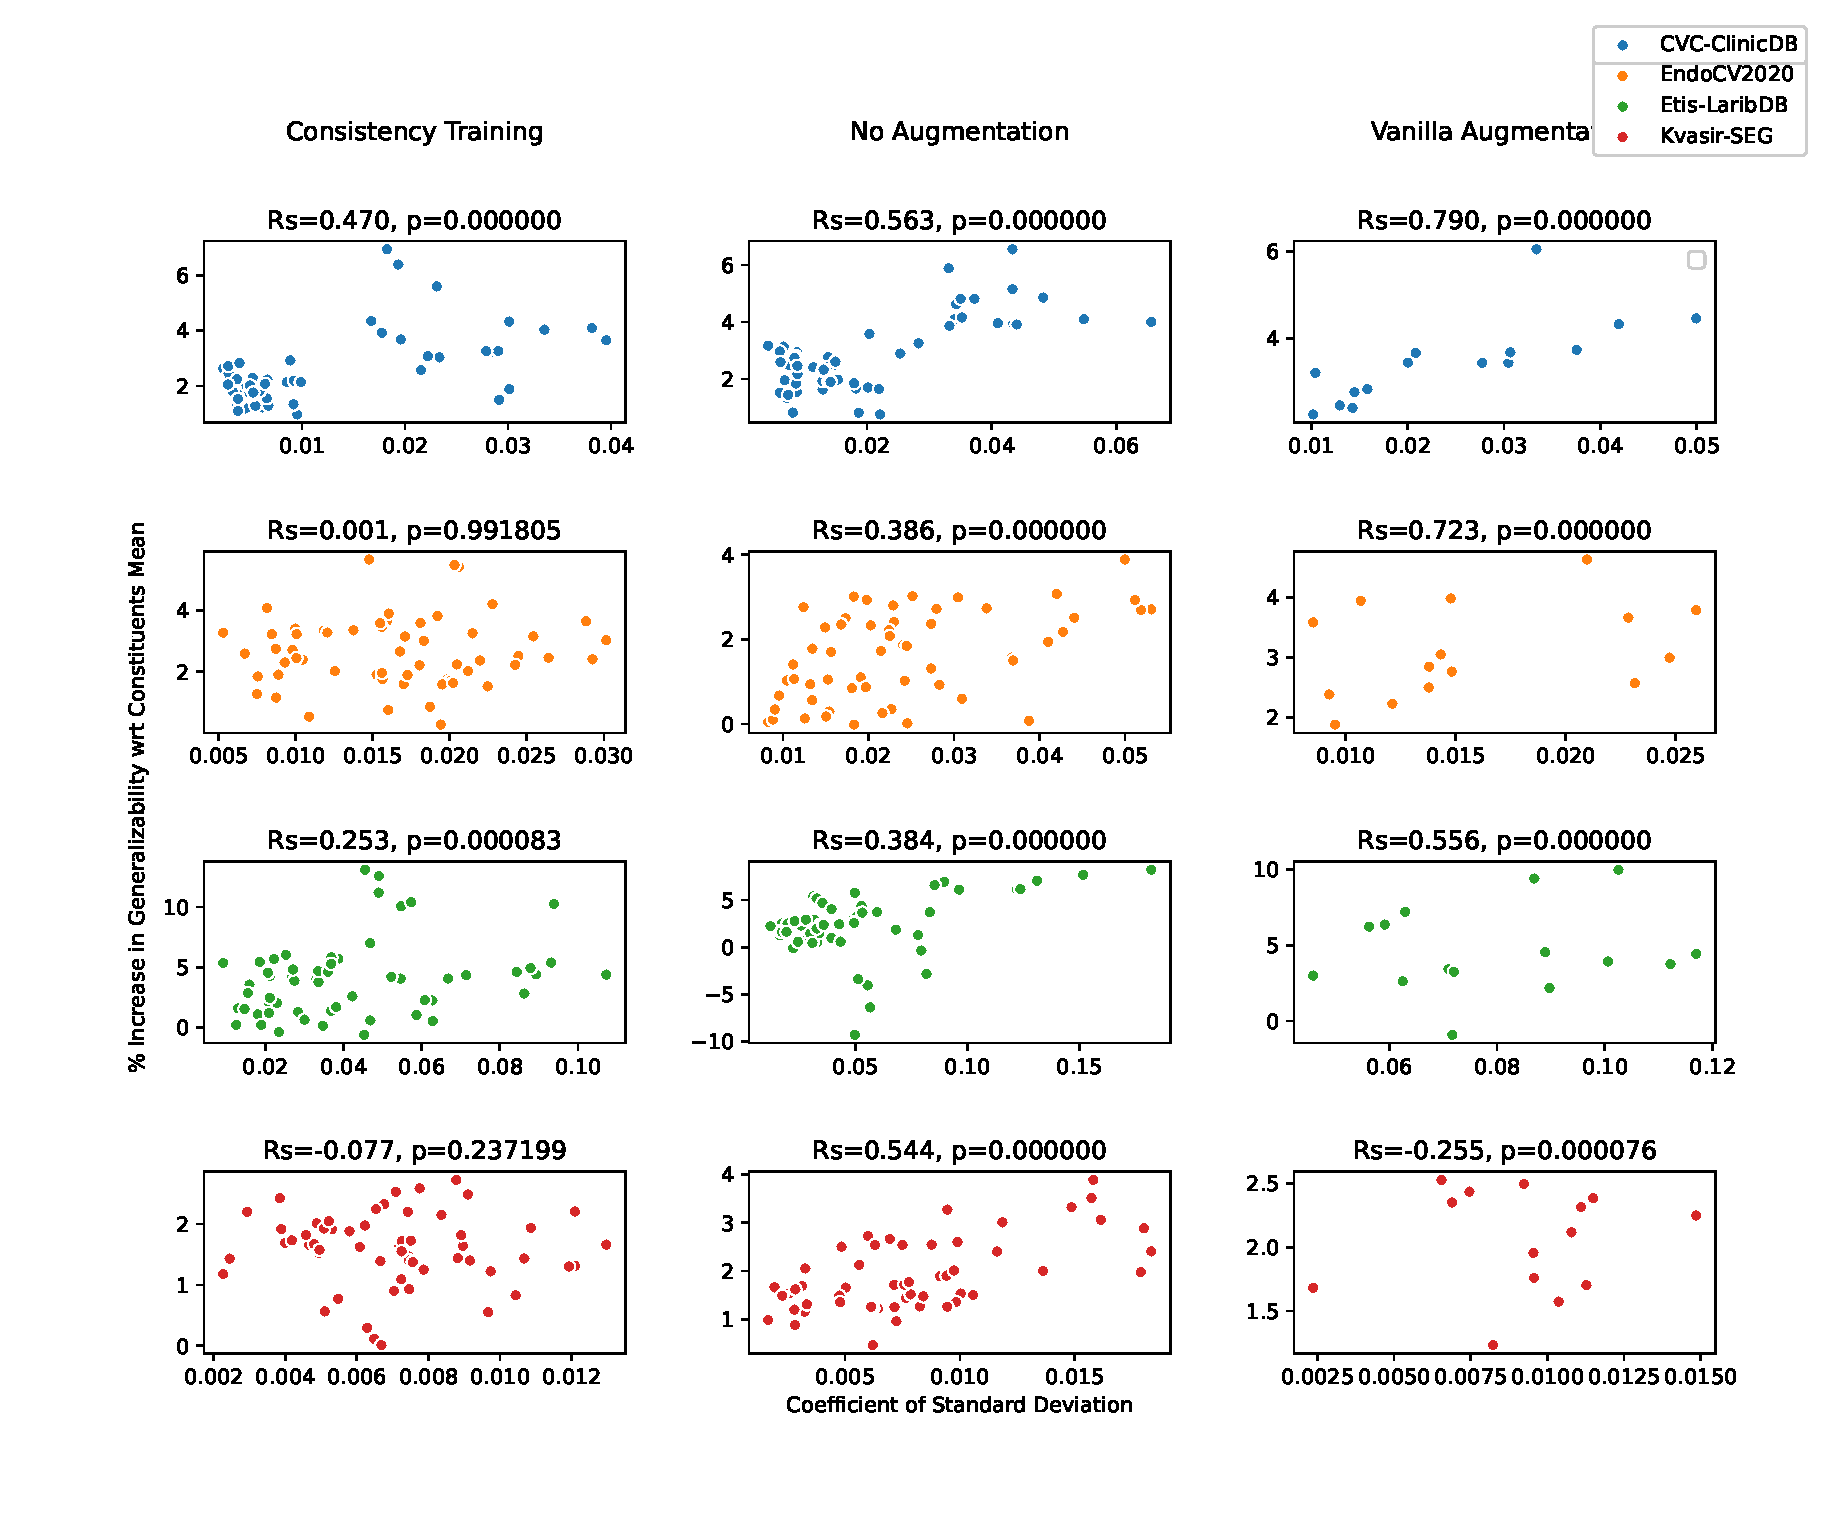
\includegraphics[width=1.2\linewidth]{illustrations/ensemble_variance_relationship_statistical.eps}
     \caption[Relationship between ensemble improvements and constituents' performance variability]{Plot showing the correlation between the improvements to \gls{iou} with respect to the mean \gls{iou} of the constituent predictors, versus the variability in the performance of the constituent predictors. The Spearman Correlation Coefficient and corresponding p-value for each dataset is shown in the title of each subplot.}
    \label{fig:ensemble_var_stat}
\end{figure}

The \gls{cs} values are in this case based on five predictors - half as many as in~\Cref{fig:ensemble_improvements}, thus there may be a larger degree of measurement error along the x-axis. Nevertheless, there overall appears to be a generally positive relationship between the ensemble constituent's \gls{cs} of \gls{iou} and the relative improvements in mean \gls{iou} due to ensembles. When the ensembles are trained either with or without conventional augmentation, this relationship is statistically significant for all datasets when comparing across all models. When trained with Consistency Training, it is statistically significant for Etis-LaribDB and CVC-ClinicDB. The weak correlation in the remaining datasets may be attributed to the fact that the models generally perform with low degrees of variability on them, as shown in \Cref{fig:consistency_cstd}. This low variability suggests that the predictors all return fairly similar segmentations, which also explains the comparatively low impact of the ensembles on these datasets.  



\section{Summary}
This chapter detailed the experiments performed to evaluate the methods presented in~\Cref{methods} along with the effects of model architecture, augmentation, and ensembles on generalizability. The results can be summarized as follows:
\begin{itemize}
    \item Model architecture had limited bearing on increasing generalization, but large models are likely to harm it.
    \item Multitask learning as implemented using the Dual-decoder DeepLabV3+ had negligible impact, which may be attributed to the encoder learning dataset-agnostic features.
    \item Data augmentation increased generalization considerably, but the use of the generative inpainter had a negative effect.
    \item Consistency Training outperformed conventional data augmentation and increased generalization by statistically significant margins.
    \item Ensembles models increased generalization. The relationship between this increase and underspecification was investigated, and shown to be positively correlated to statistical significance. 
\end{itemize}

These findings will be discussed in further detail in~\Cref{discussion} along with their impact and limitations. 
